\section{Abstract}

Efficient prediction and ranking of small molecule binders by their kinetic (\kon and \koff) and thermodynamic ($\Delta G$) properties can be a valuable metric for
drug lead optimization, as these quantities are often indicators of \textit{in vivo} efficacy.
We have
previously described a hybrid molecular dynamics, Brownian dynamics, and milestoning model, Simulation Enabled Estimation of Kinetic
Rates (SEEKR), that can predict \kon's, \koff's, and $\Delta G$'s. Here we demonstrate the effectiveness of this approach for ranking a
series of seven small molecule compounds for the model system, \bcd, based on predicted \kon's and \koff's. We compare our results using
SEEKR to experimentally determined rates as well as rates calculated using long-timescale molecular dynamics simulations and show that
SEEKR can effectively rank the compounds by \koff and $\Delta G$ with reduced computational cost. We also provide a discussion of
convergence properties and sensitivities of calculations with SEEKR to establish ``best practices'' for its future use.

\section{Introduction}

\par Molecular binding processes are ubiquitous in biology and serve as the
fundamental basis for biological complexity.
For the drug discovery community, engineering pharmacologically active small molecules is of
particular importance. Traditionally, the paradigm for lead optimization is to
select for leads with the greatest affinity for a protein, or other, target of
interest. However, recent evidence suggests that the kinetics of binding may
also be a useful metric for lead selection. It is now thought that both residence
times and association rates are key determinants of \textit{in vivo} efficacy
for many drugs\cite{Schuetz2017,Lu2010a,Copeland2006b,Copeland2016,Swinney2004b}.
Similar to computational predictions of binding thermodynamics, molecular
simulations can be used to compute binding kinetics\cite{DeVivo2016,Amaro2018,Bruce2018a}. Methods such as Brownian
Dynamics (BD) have been used effectively for estimating molecular
association rates\cite{Northrup1984,McCammon1986,Zhou1990,Huber2010}.
Molecular dynamics (MD) simulations
which explicitly represent all atoms and forces, can also be used to predict
binding kinetics. Due to significantly increased model complexity, MD is
limited by sampling. Nevertheless, owing to software improvements and the
development of commodity hardware such as GPUs and specialty hardware such as
Anton\cite{Shaw2009,Shaw2014}, ``brute force'' calculation of binding kinetics with MD is now
a possibility\cite{Shan2011,Shan2012,Dror2011,Pan2013a,Tang2017}. To improve
upon ``brute force'' sampling statistics, many sampling strategies
employ force biases or other statistical mechanical techniques to predict
both association and dissociation rates of many systems. This includes methods
such as: Markov State Models\cite{Buch2011b,Plattner2015a,Wu2016,Doerr2014},
metadynamics\cite{Mollica2016a,Tiwary2015,Casasnovas2017},
milestoning\cite{Elber2017,Ma2017,Kirmizialtin2012,Yu2015,Bucci2016,Ma2015,Ma2017},
and other techniques\cite{Teo2016,Dickson2016,Dickson2017,Lotz2018a,Chiu2016,Wong2018,Tran2018}.

\par Our previous work uses a multiscale MD, BD, and Milestoning approach for
the calculation of both association and dissociation rates of receptor-ligand
complexes\cite{Votapka2015,Votapka2017}. Our implementation, %of this simulation scheme,
``Simulation Enabled Estimation
of Kinetic Rates'' (SEEKR)
is a freely available software package\footnote{https://amarolab.ucsd.edu/seekr} that automates the preparation,
simulation, and analysis of these multiscale milestoning calculations using
existing softwares: NAMD\cite{Phillips2005} for MD simulations and
BrownDye\cite{Huber2010} for BD simulations.
Milestoning theory
provides the glue for the multiscale scheme by providing a strategy to subdivide,
simulate, and subsequently statistically reconnect small regions of simulation
space called ``milestones''\cite{Faradjian2004,Shalloway2006,West2007,Vanden-Eijnden2008,
Vanden-Eijnden2009,Majek2010,Kirmizialtin2011,Cardenas2013,Cardenas2015,
Bello-Rivas2015,Votapka2015,Votapka2017,Elber2017} This approach reduces the compute time required to simulate transition events, is embarrassingly parallel, and is agnostic to the simulation modality used.
This allows us to use atomically detailed, yet computationally expensive,
fully flexible MD simulations in milestones near the binding site where these
interactions are critical for understanding the binding and unbinding, and BD
simulations far from the binding site where rigid body dynamics provides a
sufficient description at significantly reduced computational cost. For a more
thorough description of milestoning theory and the calculation of kinetic
quantities, such as \kon and \koff, we refer the reader to the existing
literature.\cite{Faradjian2004,Shalloway2006,West2007,Vanden-Eijnden2008,
Vanden-Eijnden2009,Majek2010,Kirmizialtin2011,Cardenas2013,Cardenas2015,
Bello-Rivas2015,Votapka2015,Votapka2017,Elber2017}

\par The effectiveness of the SEEKR scheme for the calculation of \kon and \koff
values has been demonstrated for multiple protein-ligand systems\cite{Votapka2015,Votapka2017}.
However, it has not yet been used for rank ordering sets of compounds by kinetic
(\kon and \koff) and thermodynamic ($\Delta G$) values, as would be done in
pharmaceutical discovery settings. Here we use SEEKR to estimate \kon , \koff, and $\Delta G$
for a model host-guest system, $\beta$-cyclodextrin with seven ligands
representing diverse chemical groups (Fig.~\ref{fig:BCD_ligands}), using two
forcefields for $\beta$-cyclodextrin  GAFF\cite{Wang2004,Wang2006} and Q4MD\cite{Cezard2011}. We compare the SEEKR estimates with previously
published ``brute force'' (long-timescale) MD predictions\cite{Tang2017} and experimental
results\cite{Fukahori2004,Fukahori2006,Nishikawa2002,Nishikawa2006,Rekharsky1998,Barros1998}.
Using this model system we examine both the accuracy and efficiency of SEEKR compared
to long-timescale MD. We further explore the reduction in computational effort
required for SEEKR estimates as well as discuss the convergence properties and
sensitivity of SEEKR calculations to establish ``best practices'' for its future
use.

\begin{figure}
    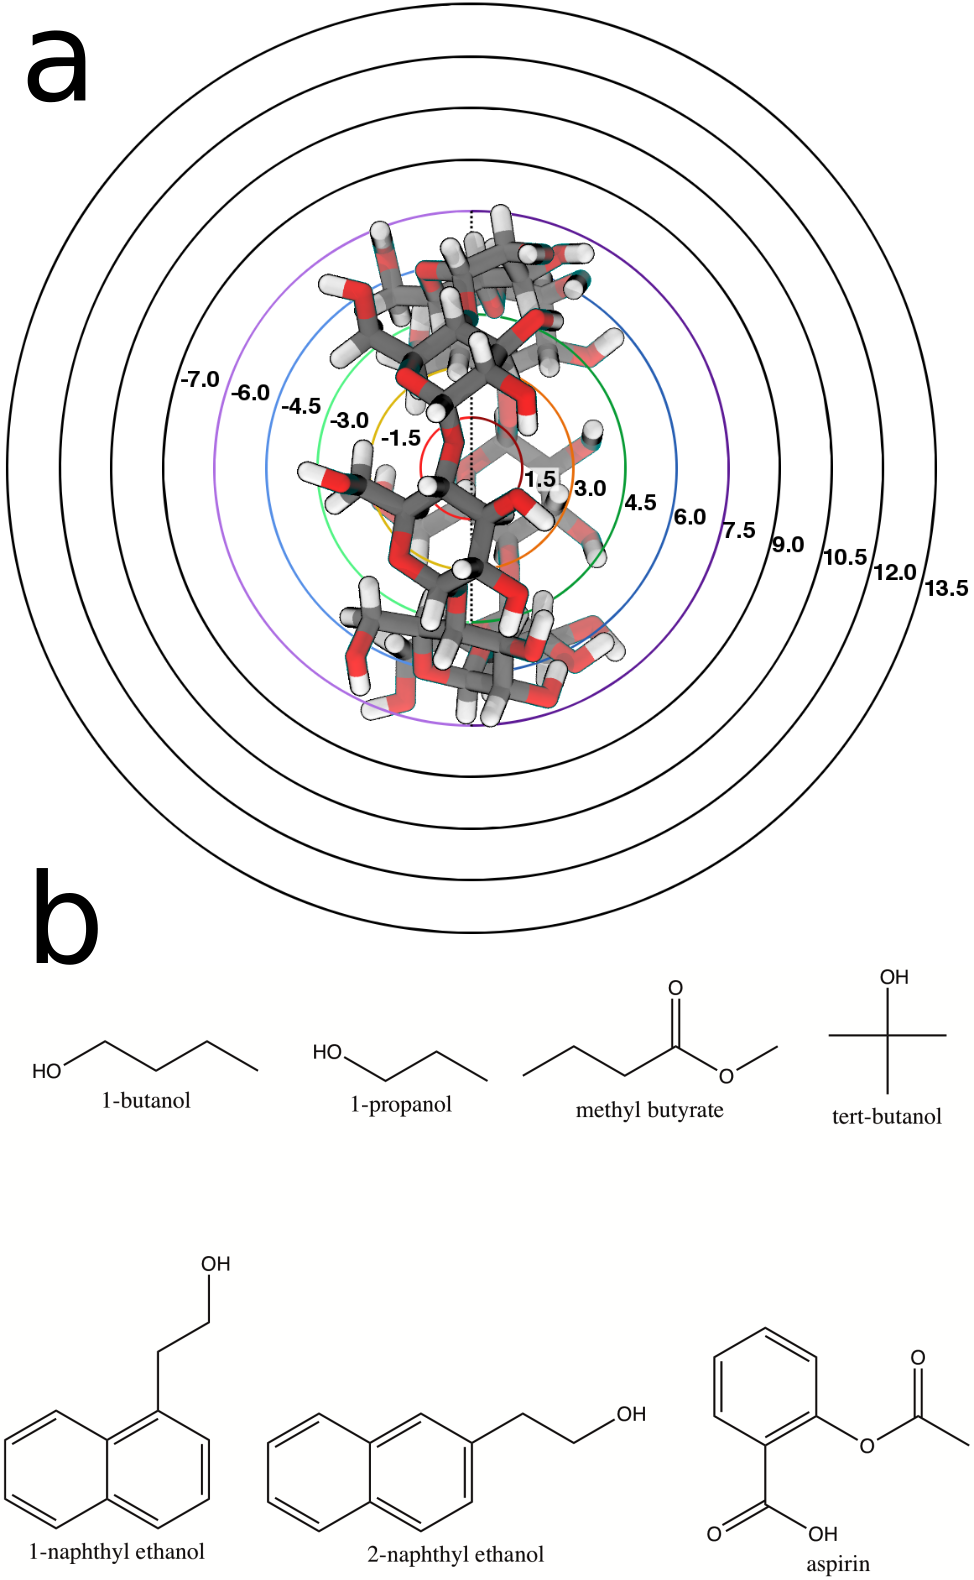
\includegraphics{images/bcdmilestones_comb_resize2.png}

	\caption{a) $\beta$-cyclodextrin with milestones spaced at 1.5~\AA increments and b) the seven ligands used in this study. The top four ligands are known to bind more weakly while the bottom three are known to bind more tightly.}
	\label{fig:BCD_ligands}
\end{figure}

\par SEEKR calculations and the long timescale MD simulations struggle to
reproduce both the values and rank ordering of the experimentally determined \kon's (Fig.~\ref{fig:on_scatter}).
\begin{figure}
	\begin{subfigure}{\linewidth}
	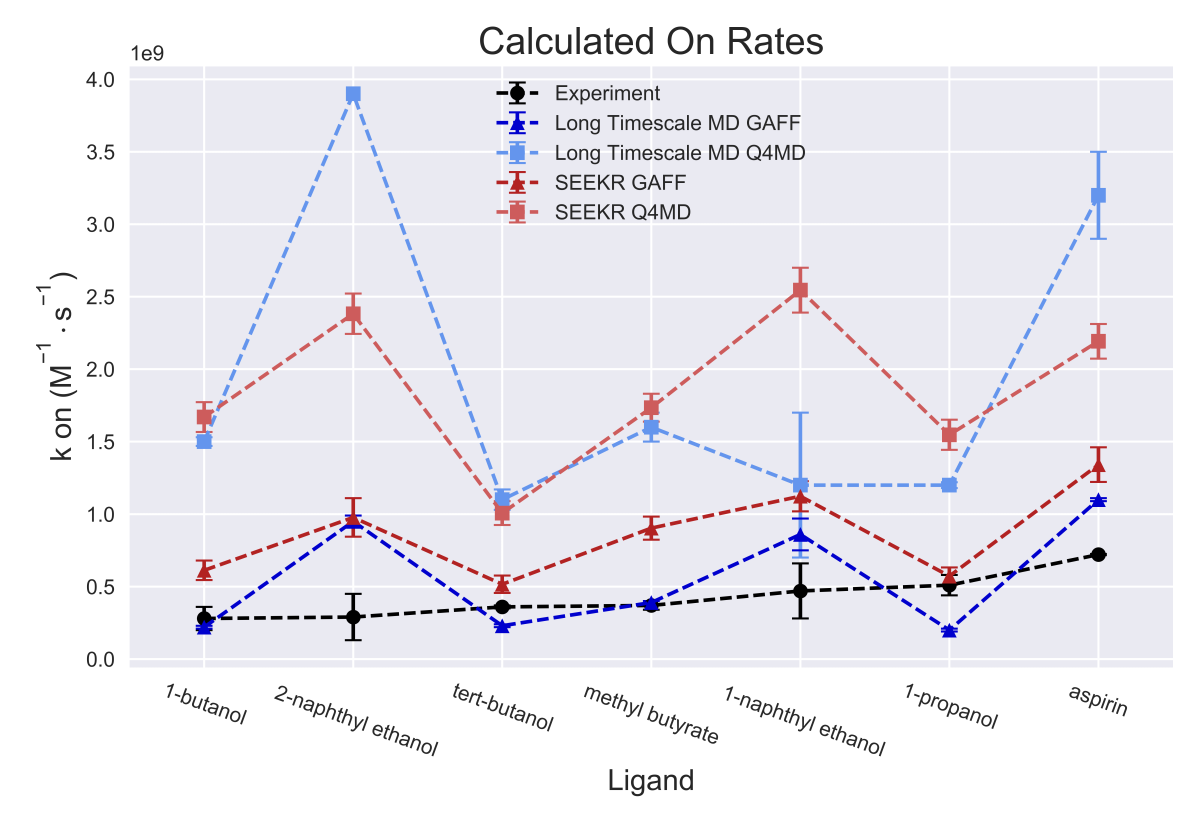
\includegraphics{images/on_scatter_resize.png}
	\caption{}
	\end{subfigure}

	\bigskip

	\begin{subfigure}{\linewidth}%<-- changed width
		%\centering
        %\renewcommand\tabularxcolumn[1]{m{#1}}% <-- added
        %\renewcommand\arraystretch{1.3}
        %\setlength\tabcolsep{2pt}% <-- added
    \begin{tabular}{
l  S[table-format = 2.3(3), separate-uncertainty]
  S[table-format = 2.3(3), separate-uncertainty]
 }%{\linewidth}%{*{4}{>{\centering\arraybackslash}X}}% <-- changed

\textbf{Method} & \textbf{Kendall} & \textbf{Spearman}  \\
\hline
      SEEKR GAFF      &    -0.20(31)           &    -0.29(40)            \\
      SEEKR Q4MD      &    0.14(29)           &    0.14(38)             \\
      Long Timescale MD GAFF      &    0.24(26)           &    0.25(29)                     \\
      Long Timescale MD Q4MD      &    0.00(28)           &    -0.05(37)                     \\


    \end{tabular}
        \caption{}
	\end{subfigure}
	\caption{a) Experimental and calculated on rates for SEEKR GAFF and Q4MD forcefields as well as long timescale MD with both forcefields. b) Calculated rank correlation coefficients. Errors are determined with a bootstrapping analysis. }
  \label{fig:on_scatter}
  \end{figure} However, similar qualitative results are seen with the SEEKR calculations and
long timescale MD calculations using the same forcefield.
On rates calculated using Q4MD are approximately one order of magnitude faster
than experimental rates, while the GAFF forcefield produces rates closer to the
experimental values, differing by approximately a factor of 3 or less.

\par Both methods fail to effectively order the ligands by increasing \kon,
as demonstrated by low or negative Kendall and Spearman rank correlation coefficients.
As the values of all the experimental rates have limited variability (all within
half an order of magnitude), the sensitivity of the methods as well as the errors
associated with the calculations and experiments makes differentiation and
ordering challenging.


\par Unlike the experimental \kon's, \koff's for the seven guest
molecules span multiple orders of magnitude, making them a better target for
ranking the compounds with SEEKR.
Again, off rates calculated with SEEKR are in good agreement with the long
timescale MD simulations using the same forcefield (Fig.~\ref{fig: off_scatter}). Rates calculated using the
GAFF forcefield are consistently faster than experiment by approximately one
order of magnitude.
\begin{figure}
	\begin{subfigure}{\linewidth}
	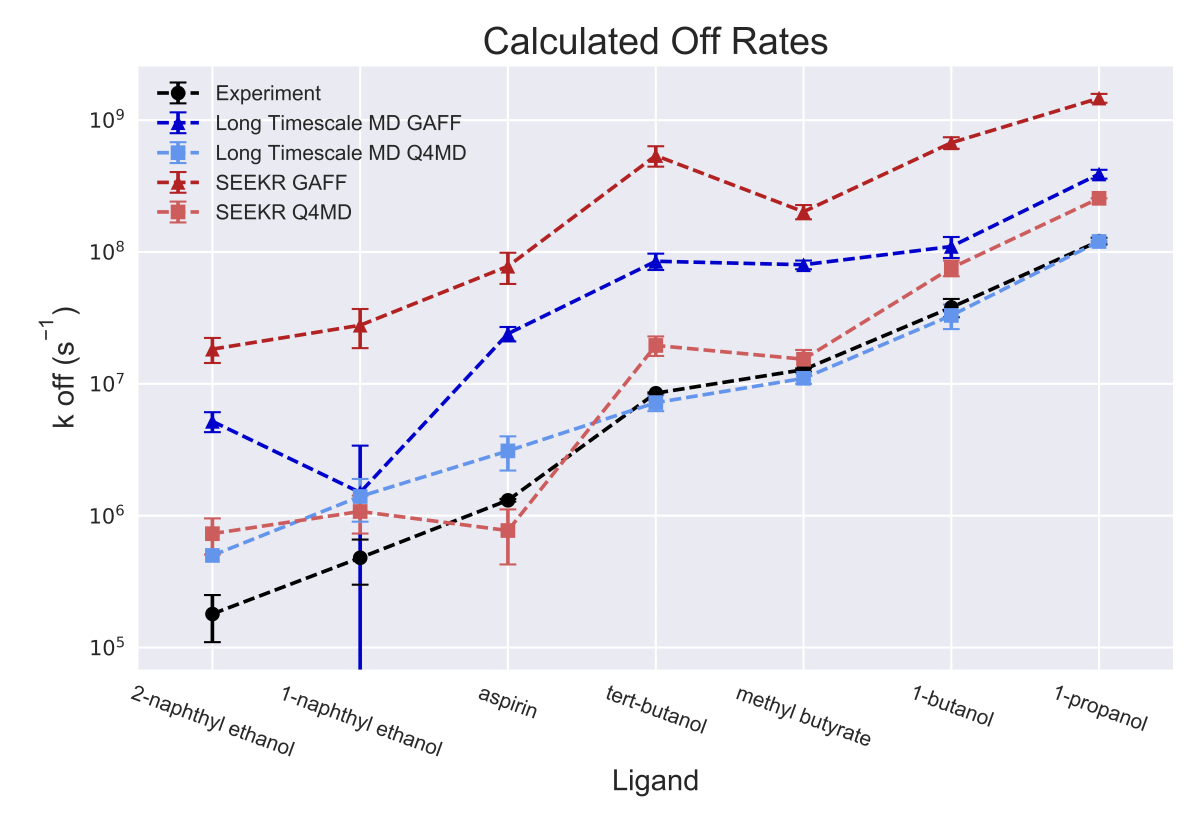
\includegraphics{images/off_scatter_resize.png}
	\caption{}
	\end{subfigure}

	\bigskip


	\begin{subfigure}{\linewidth}%<-- changed width
		%\centering
        %\renewcommand\tabularxcolumn[1]{m{#1}}% <-- added
        %\renewcommand\arraystretch{1.3}
        %\setlength\tabcolsep{2pt}% <-- added
    \begin{tabular}{
l  S[table-format = 2.3(3), separate-uncertainty]
  S[table-format = 2.3(3), separate-uncertainty]
 }%{\linewidth}%{*{4}{>{\centering\arraybackslash}X}}% <-- changed

\textbf{Method} & \textbf{Kendall} & \textbf{Spearman}  \\
\hline
      SEEKR GAFF      &    0.90(06)           &    0.96(04)            \\
      SEEKR Q4MD      &    0.81(09)           &    0.93(05)             \\
      Long Timescale MD GAFF      &    0.81(09)           &    0.93(04)                     \\
      Long Timescale MD Q4MD      &    01.00(05)           &    1.00(03)                     \\


    \end{tabular}
        \caption{}
	\end{subfigure}
	\caption{a) Experimental and calculated off rates for SEEKR GAFF and Q4MD forcefields as well as long timescale MD with both forcefields. b) Calculated rank correlation coefficients. Errors are determined with a bootstrapping analysis. }
	\label{fig: off_scatter}
\end{figure}

This trend is seen in both the long timescale MD and SEEKR,
but is more pronounced in the SEEKR calculations. The Q4MD forcefield, however,
more accurately reproduces the magnitude of the experimental values with both
SEEKR and long timescale MD. SEEKR calculations with both Q4MD and GAFF
forcefields were effective for ranking the compounds by increasing off rates, as evidenced by high rank correlation values.
The smaller magnitudes of the Q4MD
values potentially contribute to this forcefield's difficulty to differentiate
between compounds with similar rates, where the larger values associated with
the GAFF forcefield allow for more variability in the rate value without changing
the overall ordering. Both the GAFF and Q4MD forcefields successfully differentiate
the three tighter binding compounds from the four weaker binding, with the tighter binding compounds
all having slower off rates and a difference of one order of magnitude between
the fastest tightly binding compound and the slowest weakly binding compound. This suggests that SEEKR
could be useful for identifying and separating long residence time ligands from
shorter residence time ligands and then further discriminating the compounds
through ranking by \koff.


\par An additional benefit of kinetics calculations with SEEKR is that binding
free energies can also be obtained from the same simulations (Fig.~\ref{fig:dg_scatter}).

\begin{figure}
	\begin{subfigure}{\linewidth}
	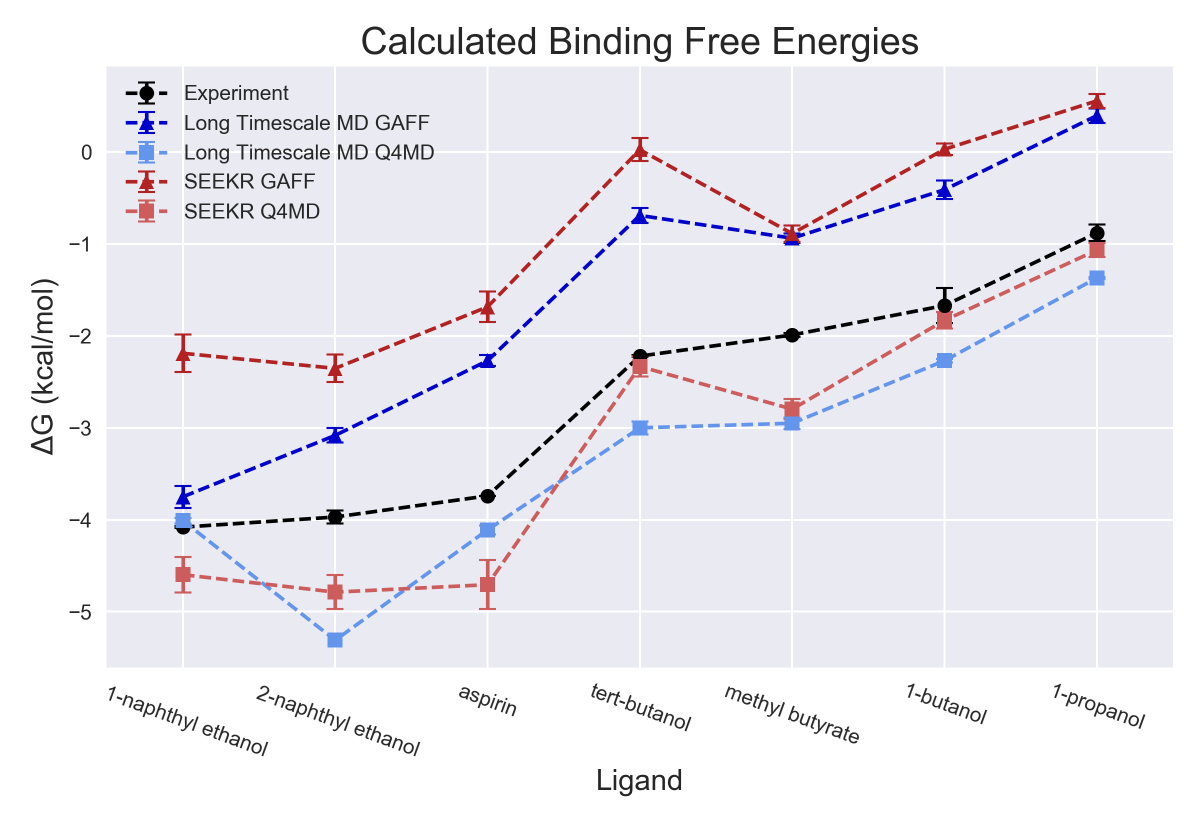
\includegraphics{images/dg_scatter_resize.png}
	\caption{}
	\end{subfigure}
	\bigskip
	\begin{subfigure}{\linewidth}%<-- changed width
		\centering
        %\renewcommand\tabularxcolumn[1]{m{#1}}% <-- added
        %\renewcommand\arraystretch{1.3}
        %\setlength\tabcolsep{2pt}% <-- added
	    \begin{tabular}{
	    	l  S[table-format = 2.3(3), separate-uncertainty]
	  		S[table-format = 2.3(3), separate-uncertainty]
	 	}%{\linewidth}%{*{4}{>{\centering\arraybackslash}X}}% <-- changed

			\textbf{Method} & \textbf{Kendall} & \textbf{Spearman}  \\
			\hline
	        SEEKR GAFF      &    0.88(08)           &    0.96(05)            \\
	        SEEKR Q4MD      &    0.73(10)           &    0.89(06)             \\
	        Long Timescale MD GAFF      &    0.90(07)           &    0.96(04)                     \\
	        Long Timescale MD Q4MD      &    0.87(11)           &    0.94(06)                     \\


	    \end{tabular}
        \caption{}
	\end{subfigure}
	\caption{a) Experimental and calculated binding free energies for SEEKR GAFF and Q4MD forcefields as well as long timescale MD with both forcefields. b) Calculated rank correlation coefficients. Errors are determined with a bootstrapping analysis. }

	\label{fig:dg_scatter}
\end{figure}

Binding free energies calculated using the rate constants
are most heavily influenced by the \koff for these ligands, as this value is more variable, where
the \kon's for all ligands are more similar. Therefore, similar trends are observed
for the calculated binding free energies as were observed for the off rates.
Binding free energies can also be calculated using the stationary probabilities
for each milestone, rather than the rate constants, and produce similar results.
The GAFF forcefield consistently underestimates the binding free energies in both
SEEKR and the long timescale MD, resulting from the consistent underestimation
of the magnitudes of the \koff's. The magnitudes of the binding free
energies calculated using Q4MD are in much better agreement with the experimental
values, differing by 1 kcal or less. SEEKR with both Q4MD and GAFF successfully
differentiates the three known tighter binding compounds from the four weaker binding compounds.
SEEKR can also further discriminate ligands
by its effective ranking %of ligands
by binding free energies, demonstrated by high rank correlation values.


\par A key aspect of future development of the SEEKR software is the systematic
development of methodological best-practices as well as the elucidation of the
sensitivity of calculated kinetic parameters to various SEEKR input conditions.

While it is possible to determine the kinetics for small systems like
$\beta$-cyclodextrin using conventional long timescale MD simulations, increasing
system size soon makes this inefficient or even impossible.
The convergence of \kon and \koff were assessed by calculating the rate
constants as a function of the reversal trajectory number at increasing intervals
of 50 reversal numbers (with 10 trajectories initiated for each reversal number).
The reversal number is a direct measure of the equilibrium simulation length, as
reversals are initiated from evenly spaced configurations of the equilibrium distribution.
In general, both the on and off rates appear converged in less than the maximum
number of reversals available. Approximately half the total reversals
(4000 of 8000) were sufficient for obtaining reasonably converged rate constants.
This suggests that the total simulation cost to obtain a similar result could be
as little as 2 ${\mu}s$ per ligand, rather than 3.8 ${\mu}s$.

\par Convergence of the rate constant is a highly complicated quantity dependent
on the transition probabilities as well as the incubation times obtained from
each milestone. Therefore, a more detailed analysis of the convergence of
these quantities on a per milestone level can provide further insight into the
overall convergence of a rate calculation within SEEKR. Fig.~\ref{fig:aspirin_conv_fig}a,b shows the convergence
of \kon and \koff, respectively, as a function of the number of reversals
launched for the representative system of Q4MD \bcd with aspirin. Reversal number is directly related to the length of
equilibrium sampling, the current bottleneck of a SEEKR
calculation.
While both values appear to converge in fewer than the maximum
number of reversals, the dramatic change in \koff after
reversal number 400 is of note. Further analysis of the
per-milestone transition counts (Fig.~\ref{fig:aspirin_conv_fig}c) and
incubation times (Fig.~\ref{fig:aspirin_conv_fig}d) revealed
that this change in \koff was due to poor initial sampling of
the -1.5 \AA milestone, which once sampled decreased the overall \koff.

\begin{figure}
	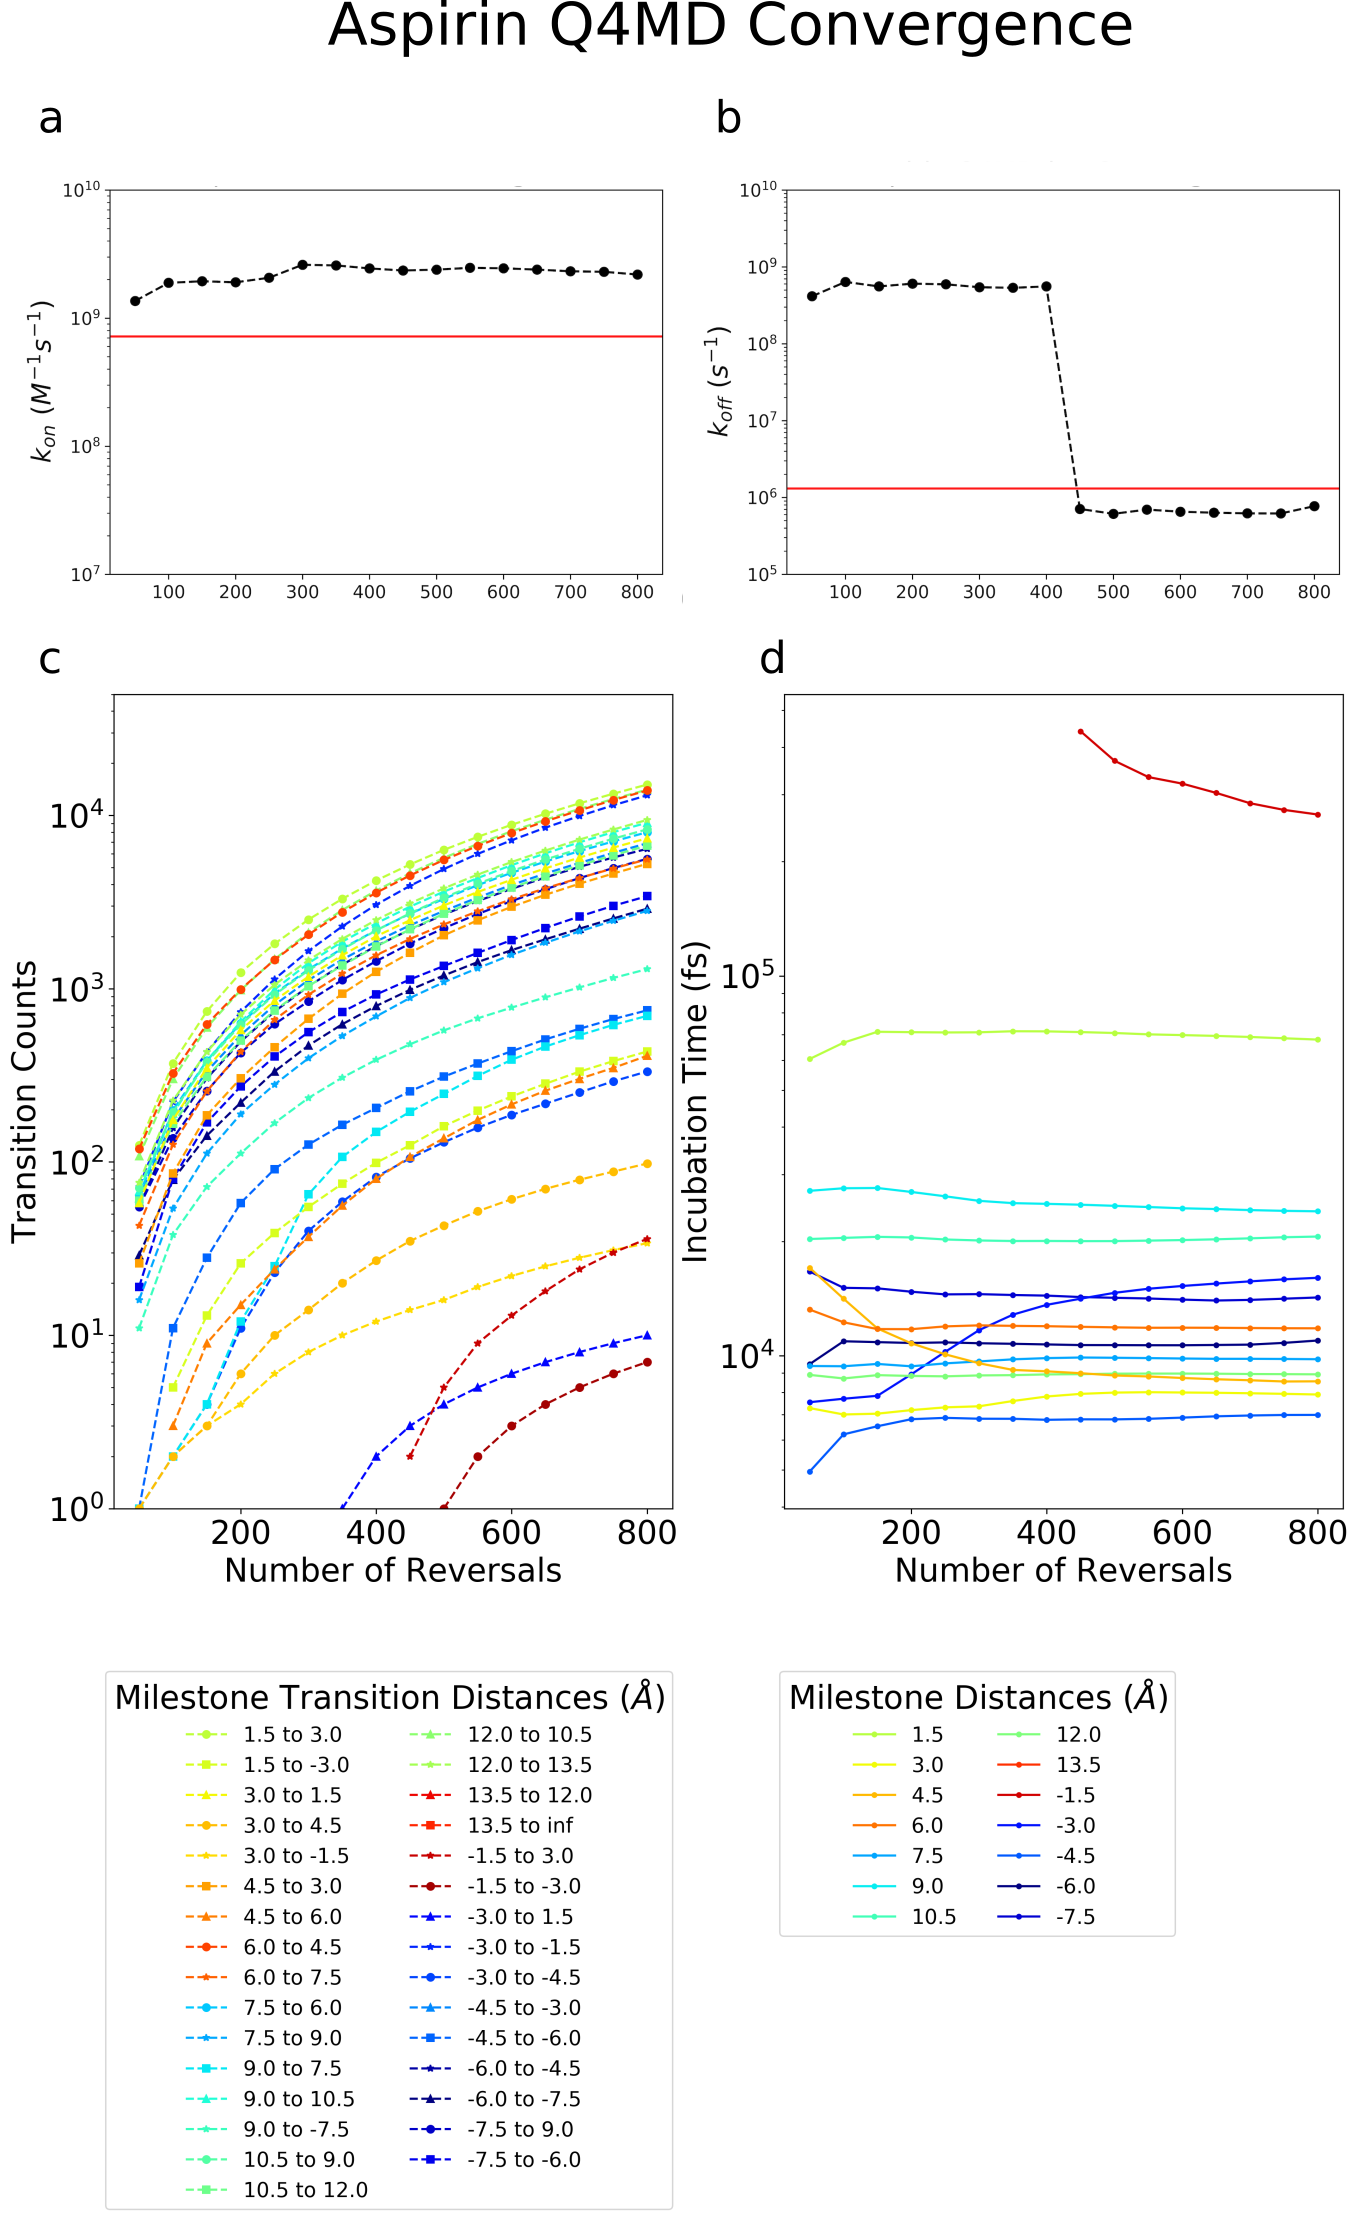
\includegraphics{images/aspirin_conv_comb.png}

	\caption{Convergence analysis for a representative ligand,  aspirin, and \bcd with the Q4MD forcefield. Convergence of a) \kon, b) \koff,  c) transition counts, and d) incubation times for each milestone are plotted as a function of the number of reversals launched.  Reversal number is directly related to the length of equilibrium sampling, as reversals were launched at 2 ns intervals from the equilibrium trajectory.}
	\label{fig:aspirin_conv_fig}
\end{figure}

This was only observed for the aspirin ligand, one of the bulkiest ligands, where it was extremely unlikely to observe transitions outward from the primary face due to steric effects.
Evaluation of these convergence properties on a
per milestone basis is a valuable diagnostic tool; identifying which
milestones contribute most to the mean first passage time (and therefore \kon
and \koff) and milestones where the ligand spends only a short time, providing
detailed molecular insight into the binding and unbinding processes.
Furthermore, this analysis is also useful during the simulation process,
as the convergence of each milestone can be assessed ``on the fly'' and individual simulations
can be terminated or extended accordingly for each milestone.

\par We also explore the sensitivity of the calculated rate constants to the milestoning model construction. In particular, the appropriate
spacing of milestones is critical for the calculation. Milestones must not be
spaced so close such that the velocity of the system cannot decorrelate between
transitions \cite{Vanden-Eijnden2008,West2007}. This assumption is typically
valid for molecular dynamics simulations, as velocities typically decorrelate on
the subpicosecond timescale \cite{Vanden-Eijnden2008}. However, if milestones are
spaced far apart, transitions will require much longer simulations and
milestioning sampling efficiency is lost.

For our systems, the incubation times of all milestones are on the order
of multiple picoseconds or greater, which
is longer than the sub-picosecond timescale typically necessary for decorrelation\cite{Vanden-Eijnden2008}.
When the milestone spacing was doubled to 3~\AA, simulation efficiency was
dramatically reduced, such that few to no transitions between milestones were
observed, precluding the calculation of rate constants. These observations suggest
that the 1.5~\AA spacing used in our simulations was appropriate for the
calculation of the desired kinetic parameters.

\par Our milestoning model differentiates the two faces
of the cyclodextrin ring and therefore defines two bound states, corresponding
to each face. Investigation into the effect of this on the resulting rate
constants revealed that it had only minimal effects. When the two bound states
were combined into a single milestone, only small changes to the rate were
observed, within the error of both calculations. Furthermore, when the the two
faces were not differentiated with unique milestones, minimal change in the
calculated rate constants was observed.

\par It is also important to note that our milestoning model did not explicitly
resolve the ligand orientation in any way, and therefore any ligand orientational
sampling was achieved entirely through simulation. This resulted in some ligand
orientations being unsampled in the deepest milestones where the orientation was
sterically restricted to the starting conformation on that milestone. While this
is a limitation that will be addressed in future developments of SEEKR, it also
highlights that a relatively simplistic model was able effectively calculate
kinetic parameters with good agreement to experimental values.

\par The simplicity of this model has many advantages. The bound state is
defined naturally as the innermost milestone and all other milestones can be
defined at the same time, including what defines the unbound state. The long
timescale MD employed a more empirical definition of the bound state where the
ligand was only considered bound when the COM of the ligand was within 7.5~\AA
of the COM of the $\beta$-cyclodextrin for at least 1.0~ns. Similarly the ligand
was considered unbound when it left this 7.5~\AA bound state for at least 1.0~ns.
With the SEEKR approach, minimal prior knowledge of the system is required, as
binding and unbinding are determined only from the milestone surfaces. No time
cutoff is required, as short excursions that do not result in full binding and
unbinding events are captured naturally in the milestoning model. The simplicity of SEEKR milestoning calculation setup, in conjunction with
the ability to monitor convergence for each milestone and terminate
simulations accordingly, makes this approach well-suited for
calculations with multiple ligands as would be necessary in a drug
discovery setting.


\par We present the first successful ranking of a set of seven guest molecules
with the $\beta$-cyclodextrin host using the SEEKR hybrid MD/BD/Milestoning approach.
SEEKR effectively reproduces both the magnitudes and rankings of the
experimental off rates\cite{Fukahori2004,Fukahori2006,Nishikawa2002,Nishikawa2006,Rekharsky1998,Barros1998} and binding free energies, two quantities of interest in
typical drug discovery campaigns\cite{Lu2010a,Schuetz2017,Copeland2006b,Copeland2016}.
%need more refs for free energy part
SEEKR also successfully differentiates the known longer residence time and
tighter binding compounds from the weaker binding compounds. Our results are also in good agreement
with previously conducted long timescale MD simulations for the same set of
ligands\cite{Tang2017}. In particular SEEKR and long timescale MD simulations
using the same forcefield (GAFF or Q4MD) exhibited similar deviations from the
experimental values, with GAFF producing consistently faster off rates than
experiment and Q4MD producing consistently faster on rates. In general both
methods and both forcefields struggled to reproduce the experimental on rate
ranking, as all ligands had very similar \kon's.
The SEEKR method requires less simulation time (3.8 ${\mu}s$ per ligand)
than the long timescale MD approach (4.5 - 11 ${\mu}s$ per ligand). Furthermore,
convergence analysis of the SEEKR calculations suggests that comparable results
could be achieved with as little as 2 ${\mu}s$ per ligand. In addition, SEEKR's
milestoning approach makes these calculations highly parallel, as the
simulations on each milestone are completely independent from all other milestones.
We also provide an analysis of the sensitivity of the SEEKR
calculations to various factors such as sampling, milestone spacing, and the
construction of the milestoning model with the intention of putting forth
``best practices'' for the use of SEEKR. SEEKR's effectiveness at ranking
compounds for this small model system suggest that it is well suited for ranking
compounds of more complex protein-ligand and protein-drug systems, where the
efficiency and enhanced sampling advantages of our multiscale MD/BD/milestoning
approach will be more apparent.


\section{Computational Methods}

\par GAFF\cite{Wang2004,Wang2006} forcefield parameters for the seven guest molecule
along with both GAFF and Q4MD-CD\cite{Cezard2011} parameterizations of $\beta$-cyclodextrin
were obtained from Tang and Chang\cite{Tang2017}. For comparison we use identical structures and
parameterizations as those used in their study. These initial structures were
used by the SEEKR software for preparation of the milestoning simulations.
The preparation procedure was the same for each of the seven guest molecules and
followed standard SEEKR protocols\cite{Votapka2017}. All systems were solvated
with TIP3P waters\cite{Jorgensen1983a}. All BD simulations were performed using the BrownDye software package\cite{Huber2010}.
Electrostatic potentials of the host and guest molecules used as inputs for the
BD simulation were calculated with APBS version 1.4\cite{Baker2001}.
A modified version of NAMD 2.12 was used for all MD simulations\cite{Phillips2005}.
For all 13 milestones in the MD region, the standard SEEKR procedure for
minimization, equilibration and simulation was followed. In total, 2.6~${\mu}s$ of equilibrium sampling (160~ns for 16 milestones) were
used and approximately 570~ns of FHPD sampling for a total of 3.2~${\mu}s$ of
simulation used in the milestoning model. The total cost per ligand (including
simulation discarded for equilibration) was therefore $\sim$3.8 ${\mu}s$.  \

\section*{Acknowledgements}
We thank Zhiye Tang and Chia-en Chang for sharing structures and parameters as
well as helpful discussions. This work is funded in part by the Director's
New Innovator Award Program NIH DP2-OD007237, the National Biomedical Computation
Resource (NBCR) NIH P41-GM103426, and the National Science Foundation through
XSEDE supercomputing resources provided via TG-CHE060073 to R.E.A. B.R.J.
and C.T.L. also acknowledge support from the NIH Molecular Biophysics
Training Program (T32-GM008326).

% \bibliography{libraryU.bib,journals_short.bib}

